\chapter{Groundwork and Fundamental Principles}
\label{ch:groundwork}

% Guideline recommended length: 8-16 pages.
% TODO: this chapter is written to explain every concept the later
% methodology chapters rely on, but it is intentionally not padded
% with generic textbook material the reader can be assumed to know.
% Expand individual sections (more depth on MPPI's cost formulation,
% a worked AMCL sensor-model example, etc.) if your supervisor's
% faculty expects a deeper literature review for a Master's thesis.

This chapter introduces the concepts and software components that the
remainder of the thesis builds on: the ROS~2 communication model
(Section~\ref{sec:ros2-model}), Ackermann steering kinematics
(Section~\ref{sec:ackermann-kinematics}), the Gazebo simulator
(Section~\ref{sec:gazebo}), SLAM via Cartographer
(Section~\ref{sec:cartographer}), the Nav2 navigation stack
(Section~\ref{sec:nav2}), the physical Quanser QCar platform
(Section~\ref{sec:qcar-platform}) and the general concept of the
sim-to-real gap (Section~\ref{sec:sim-to-real-concept}).

\section{The ROS~2 Communication Model}
\label{sec:ros2-model}

The Robot Operating System (ROS) is not an operating system in the
kernel sense. It is a middleware and tooling ecosystem for distributed
robotics software, where independent processes (\emph{nodes})
communicate by publishing and subscribing to named, typed
\emph{topics} or by calling \emph{services} for synchronous
request/response interactions. This node/topic/service nomenclature
comes from the original 2009 ROS paper \cite{quigley2009ros}. \emph{Actions},
for invoking long-running, cancellable, feedback-reporting tasks,
were a later addition, formalised as a first-class ROS~2 concept
alongside topics and services \cite{macenski2022ros2}.

The original ROS (subsequently referred to as ROS~1) relied on a
custom TCP-based transport and a single centralised \texttt{roscore}
master process for node discovery. This design was later recognised
as unsuitable for real-time, multi-robot or safety-relevant
deployments: the master is both a single point of failure and a
source of unbounded discovery latency \cite{macenski2022ros2}.

ROS~2 replaces this transport with the Data Distribution Service
(DDS), an OMG-standardised, decentralised publish-subscribe protocol
originally developed for defence and industrial real-time systems
\cite{omg2015dds}. Each ROS~2 node embeds a DDS participant and
nodes discover each other via a standardised discovery protocol
(commonly Simple Discovery Protocol, SPDP/SEDP) rather than a
central registry. Topic, service and action semantics are
implemented on top of DDS's publish-subscribe and request-reply
patterns via the ROS Middleware interface (RMW) -- an abstraction
layer that lets multiple DDS implementations, such as Fast DDS and
Cyclone DDS, serve as ROS~2's transport interchangeably
\cite{macenski2022ros2}.

DDS communication is governed per-topic by Quality of Service (QoS)
policies \cite{omg2015dds}. The two relevant here are reliability
(\texttt{RELIABLE} vs.\ \texttt{BEST\_EFFORT}) and durability
(\texttt{VOLATILE} vs.\ \texttt{TRANSIENT\_LOCAL}, the latter
retaining and re-delivering the last sample(s) to late-joining
subscribers), alongside history depth and others. A mismatch between
a publisher's and a subscriber's QoS settings can silently prevent
message delivery, even when both sides otherwise appear correctly
configured. Section~\ref{sec:monitor-goal-timing} describes one such
mismatch, encountered directly during this project's own diagnostic
tooling.

This discovery and transport layer is directly relevant to this
thesis's central architectural constraint: DDS participants must
share a compatible wire protocol version to discover and communicate
with each other at all. Chapter~\ref{ch:hardware-bridge} documents
that the QCar's factory-installed ROS~2 Dashing distribution (2019)
and this project's ROS~2 Humble development host (2022) do not, in
practice, satisfy this requirement. This mismatch is one of two
independent reasons for the TCP/JSON bridge presented there
(Section~\ref{sec:rmw-incompatibility}).

\subsection{Why DDS Discovery Incompatibilities Manifest as Silence}
\label{sec:dds-discovery-mechanism}

Understanding \emph{why} a protocol-version mismatch produces total
silence, rather than a partial or degraded connection, requires a
closer look at how two DDS participants find each other in the first
place. This is the exact mechanism Chapter~\ref{ch:hardware-bridge}'s
diagnosis exercises. This discovery mechanism and the wire protocol
it runs over is defined in a separate OMG specification from the
DCPS API specification cited above: the Real-time Publish-Subscribe
(RTPS) DDS Interoperability Wire Protocol \cite{omg2014rtps}. DDS
discovery happens in two stages.

The first stage, the Simple Participant Discovery Protocol (SPDP),
has every participant periodically multicast, by default, a small
announcement of its own existence and the network endpoints it
listens on, while listening for the equivalent announcements from
others. This is how two DDS processes on the same network first
become aware of each other, with no central broker involved.

The second stage begins once two participants know of each other via
SPDP. The Simple Endpoint Discovery Protocol (SEDP) exchanges the
finer-grained information each side needs to actually match
publishers to subscribers: topic names, data types and QoS
policies. Only after SEDP completes successfully does either side
create the local proxy objects needed to actually send or receive
user data.

A topic that exists on one side but was never successfully matched
via SEDP behaves, from the application's point of view, exactly as
if the other process did not exist. No error is raised on either
side, because DDS discovery is a best-effort background process, not
a connection attempt that can fail loudly.

Both SPDP and SEDP messages are themselves serialised using the DDS
wire protocol (RTPS -- Real-Time Publish-Subscribe), which is
versioned. A participant running an RTPS implementation that
predates a given protocol revision does not necessarily reject a
newer participant's announcement outright. Depending on exactly
which fields changed between versions, it can instead fail to parse
the announcement correctly or parse it into a form that never
completes the handshake. From the outside, this looks identical to
no announcement having arrived at all.

\begin{figure}[htbp]
  \centering
  \begin{tikzpicture}[
      participant/.style={font=\small\bfseries},
      msg/.style={-{Latex[length=2mm]}, thick},
      every node/.style={font=\footnotesize}
    ]
    \node[participant] (A) at (0,0) {Participant A};
    \node[participant] (B) at (6,0) {Participant B};
    \draw[dashed] (0,-0.3) -- (0,-7);
    \draw[dashed] (6,-0.3) -- (6,-7);

    \draw[msg] (0,-1) -- (6,-1.3) node[midway,above,sloped] {SPDP announce (multicast)};
    \draw[msg] (6,-1.8) -- (0,-2.1) node[midway,above,sloped] {SPDP announce (multicast)};
    \node[align=center] at (3,-2.6) {\itshape both participants now mutually aware};

    \draw[msg] (0,-3.3) -- (6,-3.6) node[midway,above,sloped] {SEDP: topics, types, QoS};
    \draw[msg] (6,-4.1) -- (0,-4.4) node[midway,above,sloped] {SEDP: topics, types, QoS};
    \node[align=center] at (3,-4.9) {\itshape publisher/subscriber matched (if QoS-compatible)};

    \draw[msg] (0,-5.6) -- (6,-5.9) node[midway,above,sloped] {user data (RTPS)};
    \draw[msg] (6,-6.4) -- (0,-6.7) node[midway,above,sloped] {user data (RTPS)};
  \end{tikzpicture}
  \caption[DDS discovery: SPDP and SEDP stages]{DDS discovery, in two stages, before any user data is exchanged: SPDP lets participants become mutually aware with no central broker; SEDP then matches individual publishers to subscribers by topic, type and QoS. Both stages are themselves messages on the versioned RTPS wire protocol. If either side fails to parse the other's SPDP/SEDP messages (e.g.\ due to a protocol-version mismatch), the process stops here with no error raised on either side, exactly the ``silent failure'' Section~\ref{sec:rmw-incompatibility} diagnosed on hardware.}
  \label{fig:dds-discovery}
\end{figure}

QoS policies add a second, independent way for two otherwise
discoverable endpoints to fail to exchange data -- this time by
\emph{design}, not by defect. DDS defines an explicit compatibility
rule per policy, evaluated during SEDP matching: a subscriber may
request a QoS \emph{no stronger} than what a publisher offers
(Table~\ref{tab:qos-compatibility}) \cite{omg2015dds}. A subscriber
requesting a stronger policy than the publisher offers on that
dimension is a declared incompatibility. DDS silently does not
match that pair. Again, an application-level developer would learn
nothing about this without independently comparing the two sides'
QoS settings.

\begin{table}[htbp]
  \centering
  \caption{QoS compatibility rule for the two policies relevant to this thesis (strongest requestable value shown first).}
  \label{tab:qos-compatibility}
  \begin{tabular}{@{}lll@{}}
    \toprule
    Policy & Publisher offers & Subscriber may request \\
    \midrule
    Reliability & \texttt{RELIABLE} & \texttt{RELIABLE} or \texttt{BEST\_EFFORT} \\
    Reliability & \texttt{BEST\_EFFORT} & \texttt{BEST\_EFFORT} only \\
    Durability & \texttt{TRANSIENT\_LOCAL} & \texttt{TRANSIENT\_LOCAL} or \texttt{VOLATILE} \\
    Durability & \texttt{VOLATILE} & \texttt{VOLATILE} only \\
    \bottomrule
  \end{tabular}
\end{table}

By this rule, a \texttt{VOLATILE} subscriber against a
\texttt{TRANSIENT\_LOCAL} publisher is formally compatible. This is
exactly the configuration Section~\ref{sec:monitor-goal-timing}
found, on QCar, delivering zero messages in practice
despite being spec-compliant.

Section~\ref{sec:monitor-goal-timing} discusses the likely practical
reason. Durability governs whether \emph{historical}, already-published
samples are replayed to a late-joining subscriber, not merely
whether future ones are delivered. A \texttt{VOLATILE} subscriber
that joins after a transient-local publisher's relevant samples were
already sent may receive none of the backlog and then simply waits
for a next sample -- one that, for a low-frequency topic like action
status, may not arrive for a long time.

The point for this chapter is the general one: formal QoS
compatibility, as defined by the DDS specification, is a necessary
but not sufficient condition for an application to actually observe
the message flow it expects.

\subsection{The Action Interface and Goal Lifecycle}
\label{sec:action-lifecycle}

Nav2's \texttt{navigate\_to\_pose} interface, used throughout
Chapter~\ref{ch:nav-integration}, is a ROS~2 \emph{action}
\cite{macenski2022ros2}. Rather than being a distinct transport, an
action is built on top of topics and services: it pairs a
goal-request service call with two topics the server publishes on. A
feedback topic carries periodic progress updates. A status topic
reports each known goal's current state as one of a fixed
enumeration (\texttt{ACCEPTED}, \texttt{EXECUTING},
\texttt{CANCELING}, \texttt{SUCCEEDED}, \texttt{CANCELED},
\texttt{ABORTED}, among others).

The status topic uses \texttt{TRANSIENT\_LOCAL} durability, the same
property discussed above. This lets a subscriber that starts
listening partway through a goal's execution recover its current
state from the retained history, rather than being blind until the
next status change.

Status updates are only published when the server's internal state
machine actually transitions. The status topic's history depth
is finite. This means a fast state machine can advance through more
than one transition between two publishes that an external observer
actually receives. There is no guarantee that every individual state
is observable -- only that the \emph{latest} state at any polling
instant is correct.

Section~\ref{sec:monitor-goal-timing} documents exactly this: a goal
was observed to skip directly from absent to \texttt{EXECUTING} in
one status message, with no separately observable \texttt{ACCEPTED}
update in between. The server's internal state machine does pass
through \texttt{ACCEPTED} on its way to \texttt{EXECUTING} -- the
transition happened, but no status publish was ever emitted while it
was current in isolation. This is a general property of polling a
periodically published state summary, not a special case of this one
topic.

\section{Ackermann Steering Kinematics}
\label{sec:ackermann-kinematics}

The QCar is a rear-wheel-drive vehicle with front-wheel Ackermann
steering \cite{snider2009pathtracking}. The two front wheels pivot
independently about near-vertical steering axes, such that for any
commanded steering angle, both front wheels' instantaneous velocity
vectors are perpendicular to lines drawn through a single common
point on the extended rear axle. This point is the vehicle's
instantaneous centre of rotation. This geometric constraint means the
two front wheels must generally be steered to slightly different
angles, with the inner wheel turning more sharply than the outer, so
that all four wheels roll without slipping through a common turn
centre.

For control and estimation purposes, this thesis follows the
standard simplification to a single-track bicycle model
\cite{snider2009pathtracking}, which replaces the two front wheels with
a single virtual wheel at the centre of the front axle steered at
angle $\delta$ and the two rear wheels with a single virtual wheel
at the centre of the rear axle. With vehicle heading $\theta$,
wheelbase $L$ (the longitudinal distance between the front and rear
axles) and rear-axle speed $v$, the kinematic bicycle model is:

\begin{align}
  \dot{x} &= v \cos\theta \label{eq:bicycle-x}\\
  \dot{y} &= v \sin\theta \label{eq:bicycle-y}\\
  \dot{\theta} &= \frac{v}{L}\tan\delta \label{eq:bicycle-theta}
\end{align}

and the corresponding instantaneous turning radius about the rear
axle is

\begin{equation}
  R = \frac{L}{\tan\delta}. \label{eq:bicycle-radius}
\end{equation}

Equation~\ref{eq:bicycle-theta} is the basis of the onboard bridge's
dead-reckoning odometry described in Chapter~\ref{ch:hardware-bridge},
which genuinely integrates wheel-encoder and commanded-steering
readings forward through this relationship at every control cycle to
estimate pose from scratch. A single-track model is a simplification: it assumes no lateral tyre
slip and treats both front wheels as a single steering angle rather
than the true Ackermann-differentiated pair. Chapter~\ref{ch:calibration}
presents direct evidence of where this simplification's limits were
reached in practice on QCar
(Section~\ref{sec:deadband-discovery}).

\subsection{The True Two-Wheel Ackermann Angle}
\label{sec:true-ackermann}

The single-track model above is a control- and estimation-time
convenience. It is not what the Gazebo drive plugin actually
commands at the level of the two physical front wheels.

Because the two front wheels steer about laterally separated axes, a
single-track model's one steering angle $\delta$ must generally be
converted into two slightly different angles, with the inner wheel
(on the side the vehicle is turning toward) steered more sharply than
the outer. This ensures both front wheels' rolling directions remain
tangent to circles sharing the same centre on the extended rear axle.
This is the condition for rolling without slipping introduced in
Section~\ref{sec:ackermann-kinematics}'s opening paragraph. With
track width $T$ (the lateral distance between
the two front steering axes) and wheelbase $L$, the exact left- and
right-wheel steering angles corresponding to a single-track angle
$\delta$ are:

\begin{align}
  \delta_{\text{left}} &= \operatorname{atan2}\!\left(\tan\delta,\ 1 - \dfrac{T}{2L}\tan\delta\right) \label{eq:ackermann-left}\\
  \delta_{\text{right}} &= \operatorname{atan2}\!\left(\tan\delta,\ 1 + \dfrac{T}{2L}\tan\delta\right) \label{eq:ackermann-right}
\end{align}

(signed so that a positive $\delta$, a left turn, gives
$\delta_{\text{left}} > \delta_{\text{right}}$ -- the inside wheel of
the turn steers further). This is precisely the pair of relationships
the \texttt{gazebo\_ros\_ackermann\_drive} plugin evaluates every
simulation step from a single commanded angular velocity.
Chapter~\ref{ch:sim-stack} also refers to this same formula when
describing the plugin auto-computing Ackermann geometry from URDF
joint positions:
$T$ and $L$ in Equations~\ref{eq:ackermann-left}--\ref{eq:ackermann-right}
are measured directly from the URDF's own front-hub joint origins at
spawn time, never stated as separate configuration values.

As $T \to 0$ (a vanishingly narrow front track), both angles converge
to the single-track $\delta$. This confirms
Equations~\ref{eq:ackermann-left}--\ref{eq:ackermann-right} correctly
generalise, rather than contradict, the simpler model of
Equations~\ref{eq:bicycle-x}--\ref{eq:bicycle-theta}.

\begin{table}[htbp]
  \centering
  \caption{QCar Ackermann geometry parameters used throughout this thesis.}
  \label{tab:qcar-geometry}
  \begin{tabular}{@{}lll@{}}
    \toprule
    Parameter & Value & Source \\
    \midrule
    Wheelbase $L$ & \SI{0.25725}{\meter} & URDF joint geometry (measured) \\
    Front track width & \SI{0.1118}{\meter} & URDF joint geometry (measured) \\
    Rear track width & \SI{0.1122}{\meter} & URDF joint geometry (measured) \\
    Wheel radius & \SI{0.033}{\meter} & Wheel mesh bounding box (measured) \\
    Max.\ steering angle $\delta_{max}$ & \SI{0.5236}{\radian} (\ang{30}) & Vehicle/plugin limit \\
    Min.\ turning radius (from Eq.~\ref{eq:bicycle-radius}) & \SI{0.446}{\meter} & Derived \\
    \bottomrule
  \end{tabular}
\end{table}

\begin{figure}[htbp]
  \centering
  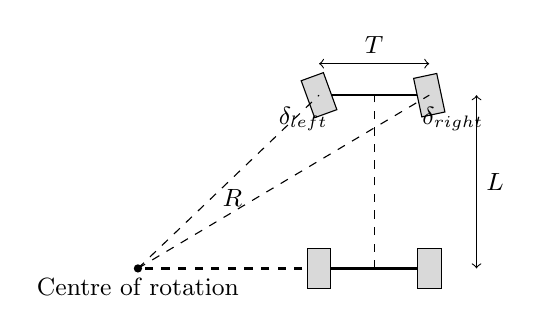
\begin{tikzpicture}[scale=1.0, every node/.style={font=\small}]
    \coordinate (RL) at (-0.7,0);
    \coordinate (RR) at (0.7,0);
    \coordinate (FL) at (-0.7,2.2);
    \coordinate (FR) at (0.7,2.2);
    \coordinate (C) at (-3.0,0);

    \draw[thick] (RL) -- (RR);
    \draw[thick] (FL) -- (FR);
    \draw[thick,dashed] (RL) -- (C);
    \draw[dashed] (0,0) -- (0,2.2);

    \draw[fill=gray!30] (RL) ++(-0.15,-0.25) rectangle ++(0.3,0.5);
    \draw[fill=gray!30] (RR) ++(-0.15,-0.25) rectangle ++(0.3,0.5);

    \begin{scope}[rotate around={20:(FL)}]
      \draw[fill=gray!30] (FL) ++(-0.15,-0.25) rectangle ++(0.3,0.5);
    \end{scope}
    \begin{scope}[rotate around={12:(FR)}]
      \draw[fill=gray!30] (FR) ++(-0.15,-0.25) rectangle ++(0.3,0.5);
    \end{scope}

    \fill (C) circle (1.5pt);
    \node[below] at (C) {Centre of rotation};

    \draw[dashed] (C) -- (FL);
    \draw[dashed] (C) -- (FR);

    \draw[<->] (1.3,0) -- (1.3,2.2) node[midway,right] {$L$};
    \draw[<->] (-0.7,2.6) -- (0.7,2.6) node[midway,above] {$T$};

    \node at (-0.9,1.9) {$\delta_{\text{left}}$};
    \node at (1.0,1.9) {$\delta_{\text{right}}$};
    \node at (-1.8,0.9) {$R$};
  \end{tikzpicture}
  \caption[Ackermann steering geometry]{Ackermann steering geometry (top-down view, not to scale): the two front wheels are steered to different angles $\delta_{\text{left}} > \delta_{\text{right}}$ (left turn shown) so that lines through both front wheels' rolling directions and the rear axle all intersect at a single centre of rotation. Wheelbase $L$ and track width $T$ are the parameters of Equations~\ref{eq:ackermann-left}--\ref{eq:ackermann-right}.}
  \label{fig:ackermann-geometry}
\end{figure}

\section{Simulation with Gazebo}
\label{sec:gazebo}

Gazebo is a physics-based 3D robot simulator, originally built around
a rigid-body dynamics engine, a small set of sensor models (odometry,
ray-proximity/laser range-finding and camera) and a modular
client/interface layer for injecting control logic into simulated
models without coupling that logic to the physics engine itself
\cite{koenig2004gazebo}.

Two later generations of Gazebo are relevant to this project's
history. Both are architecturally distinct from each other and both
extend the original model with a formal SDF-based plugin system and a
substantially wider sensor suite, including LiDAR and IMU sensor
models. Only the LiDAR model is actually used in this project's
simulation stack (see the IMU note in
Section~\ref{sec:qcar-platform}). \emph{Gazebo Classic} (versions up
to 11) integrates with ROS~2 through the separate
\texttt{gazebo\_ros} / \texttt{gazebo\_plugins} packages, while the
newer \emph{Gazebo Sim} (formerly Ignition Gazebo) integrates through
\texttt{ros\_gz\_sim} / \texttt{ros\_gz\_bridge}.

The two are not drop-in replacements for each other. Plugin
filenames, topic remapping mechanisms and world-file (SDF) syntax
for built-in physics/sensor systems all differ between them. A
package written against one will not load under the other without a
systematic conversion.

This project uses Gazebo Classic~11 with the \texttt{gazebo\_ros}
family of plugins, matching the ROS~2 Humble / Ubuntu 22.04 host
environment, in which Gazebo Sim's binaries are not available at
all.

The robot itself is described in the Unified Robot Description
Format (URDF), an XML dialect specifying the vehicle's kinematic
tree (links and joints), visual meshes and collision geometry. A
\texttt{<gazebo>} block within the URDF attaches simulation-only
elements: sensor definitions and the drive plugin
(\texttt{libgazebo\_ros\_ackermann\_drive.so}) that subscribes to
\texttt{/cmd\_vel} and converts commanded linear/angular velocity
into per-wheel drive and steering-hub joint efforts. It uses the
Ackermann geometry of Section~\ref{sec:ackermann-kinematics} for
this, auto-computed from the URDF's own joint and collision geometry
at spawn time rather than restated in a separate configuration file.

A recurring practical property of this plugin, directly relevant to
Chapter~\ref{ch:sim-stack}, is that its wheel-radius auto-detection
only supports primitive collision shapes (cylinders, spheres). A
mesh-shaped wheel collision silently yields a wheel radius of zero,
which propagates as a division-by-zero into the plugin's velocity
PID controller.

Simulated friction is likewise not automatic: both the wheel links
and the ground plane must be assigned explicit Coulomb friction
coefficients (SDF's \texttt{mu1}/\texttt{mu2}) or the simulated
vehicle exhibits perfect wheel slip with no resulting translation,
regardless of commanded wheel speed. Neither failure mode raises an
error. Both look, from the outside, like ``the robot is not
moving.'' Both are addressed in detail in
Section~\ref{sec:not-moving-bug}.

\subsection{The Plugin's PID Control Loop and the Physics Step}
\label{sec:gazebo-pid-loop}

The drive plugin does not run on its own timer. It registers a
callback on Gazebo's \texttt{WorldUpdateBegin} event, which fires
once per physics step of the rigid-body solver -- by default
\SI{1}{\milli\second} of simulated time per step, i.e.\
\SI{1000}{\hertz}, independent of and generally much faster than any
ROS~2 topic rate in the system.

On every physics step, regardless of whether a new
\texttt{/cmd\_vel} message has arrived, the callback re-reads the
rear wheel's current angular velocity from the physics engine. It
compares that reading against the most recently \emph{commanded}
linear velocity, converted to an equivalent target angular velocity
($\text{target\_linear} / \text{wheel\_radius}$) and passes the
resulting error through a discrete PID controller. The controller's
output is applied directly as a joint \emph{force} (torque), not a
velocity: this is a torque-controlled velocity-tracking loop, not a
kinematic teleport of the wheel to a commanded speed. The controller
update takes the classical form \cite{astrom2008feedback}

\begin{equation}
  u(t) = K_p\, e(t) + K_i \int_0^t e(\tau)\, \mathrm{d}\tau + K_d \frac{\mathrm{d}e(t)}{\mathrm{d}t},
  \qquad e(t) = \text{measured}(t) - \text{target}(t),
  \label{eq:pid}
\end{equation}

evaluated once per physics step, with the integral and derivative
terms accumulated or estimated over the actual, possibly
non-uniform, time elapsed since the previous step. The integral term
can optionally be clamped to a configured $[i_{\min}, i_{\max}]$
range, to prevent unbounded windup while the system is far from its
target.

Three independent instances of this controller run inside the
plugin: one for the rear-axle drive velocity and one each for the
left and right steering hubs, tracking the two Ackermann angles of
Equations~\ref{eq:ackermann-left}--\ref{eq:ackermann-right}
independently rather than as a single shared steering command. All
three sets of gains ($K_p$, $K_i$, $K_d$) are declared per-vehicle in
the URDF's \texttt{<gazebo>} plugin block. Section~\ref{sec:not-moving-bug}
documents in detail what happens when these gains are tuned for one
physical configuration (e.g.\ frictionless wheels) and then reused
unchanged after that configuration changes.

Equation~\ref{eq:pid} also explains precisely why the wheel-radius
defect above is destructive rather than merely inaccurate. With
$\text{wheel\_radius} = 0$, the target angular velocity
$\text{target\_linear}/\text{wheel\_radius}$ is not merely wrong --
it is unbounded for any nonzero commanded linear velocity. That
makes $e(t)$ itself unbounded, driving the PID controller to its
output saturation limit (or to a floating-point infinity/NaN)
regardless of how the three gains are tuned. No amount of gain
retuning can compensate for an error signal that is not a finite
number in the first place, which is why this class of bug survives
naive ``just tune the PID harder'' troubleshooting.

\begin{figure}[htbp]
  \centering
  \begin{tikzpicture}[
      block/.style={draw, rectangle, minimum height=1.1cm, text width=2.4cm, align=center, font=\small},
      sum/.style={draw, circle, minimum size=0.6cm, font=\small, inner sep=0pt},
      arr/.style={-{Latex[length=2mm]}, thick},
      node distance=1.5cm
    ]
    \node[block] (cmd) at (0,0) {Commanded\\\texttt{/cmd\_vel}};
    \node[sum] (sum) at (3.9,0) {$\Sigma$};
    \node[block] (pid) [right=of sum] {PID\\(Eq.~\ref{eq:pid})};
    \node[block] (plant) [right=of pid] {Physics step\\(rigid-body solver)};

    \draw[arr] (cmd) -- (sum) node[midway,above] {target $\omega$};
    \draw[arr] (sum) -- (pid) node[midway,above] {$e(t)$};
    \draw[arr] (pid) -- (plant) node[midway,above] {joint torque};

    \draw[arr] (plant.south) -- ++(0,-1.6) -| (sum.south);
    \node[below] at ($(pid.south)+(0,-1.6)$) {measured $\omega$};

    \node at ($(sum.north west)+(0.08,-0.05)$) {\scriptsize $+$};
    \node at ($(sum.south)+(0.25,0.12)$) {\scriptsize $-$};
  \end{tikzpicture}
  \caption[The drive plugin's per-wheel PID control loop]{The drive plugin's per-wheel torque control loop, re-evaluated every Gazebo physics step (\SI{1}{\kilo\hertz}): a commanded velocity is converted to a target angular velocity, compared against the physics engine's own measured wheel angular velocity to form an error $e(t)$ and passed through Equation~\ref{eq:pid}'s PID controller, whose output is applied directly as a joint torque. Three independent instances of this loop run per vehicle (drive, left steering, right steering).}
  \label{fig:pid-loop}
\end{figure}

\subsection{Contact Friction via the Coulomb Model and Friction Cone}
\label{sec:friction-theory}

Gazebo Classic's default physics engine, the Open Dynamics Engine
(ODE), models contact friction at each collision point using a
Coulomb friction approximation \cite{oderelease}: the maximum
tangential (sliding) force a contact can sustain before slipping is
proportional to the normal (compressive) force pressing the two
surfaces together, with the constant of proportionality being the
friction coefficient $\mu$. ODE further allows this coefficient to be
specified separately along two orthogonal directions in the contact
plane (\texttt{mu1}/\texttt{mu2} in the URDF/SDF). A tyre could in
principle grip differently along its rolling direction than sideways
across it, though this project sets both equal -- isotropic
friction. ODE itself approximates the true (circular)
Coulomb friction cone in one of two ways: a default ``constant-force-limit''
mode, where $\mu$ is treated as an absolute force limit independent
of the actual normal force or a more physically accurate ``friction
pyramid'' approximation, enabled via the \texttt{dContactApprox1}
contact flag \cite{oderelease}. This project does not override
either setting. The URDF's \texttt{<gazebo>} friction blocks
(Listing~\ref{lst:wheel-collision-friction}) set only
\texttt{mu1}/\texttt{mu2}, leaving Gazebo Classic's own default
friction-approximation mode in effect. The isotropic $\mu=1.0$ value
chosen is what actually mattered for fixing the zero-friction bug
below, not which of the two approximation modes was active.

Critically, \textbf{ODE applies no friction at all to a contact whose
$\mu_1$/$\mu_2$ default to zero}. There is no implicit ``reasonable
default'' friction coefficient assumed for an unconfigured surface,
unlike, say, a default coefficient of restitution.

This is precisely why Section~\ref{sec:not-moving-bug}'s bug~2 (zero
wheel friction) produces literal, total 100\% slip rather than
merely reduced traction. With $\mu = 0$, the Coulomb limit on
tangential force is zero regardless of how hard the wheel presses
into the ground. No sliding friction force can develop at all, no
matter how fast the wheel itself spins, so no forward thrust on the
chassis can develop either.

\section{Simultaneous Localization and Mapping with Cartographer}
\label{sec:cartographer}

Simultaneous Localization and Mapping (SLAM) is the problem of
building a map of an unknown environment while concurrently
estimating the robot's pose within that same map, using only the
robot's own sensor stream and (optionally) odometry
\cite{cadena2016slam}. This thesis uses
Google's Cartographer \cite{hess2016cartographer}, a real-time 2D/3D
LiDAR SLAM system that performs local scan matching to build
submaps and a global pose-graph optimisation to detect and correct
loop closures. It is exposed to ROS~2 via the
\texttt{cartographer\_ros} package.

Cartographer can either fuse external odometry into its
scan-matching prediction or perform scan-matching-only pose
estimation (\texttt{use\_odometry: false}). In the latter case, it
also provides the full \texttt{map} $\rightarrow$ \texttt{odom}
$\rightarrow$ \texttt{base} transform (TF) chain itself
(\texttt{provide\_odom\_frame: true}), rather than expecting an
external odometry source to supply the \texttt{odom} $\rightarrow$
\texttt{base} portion.

This configuration choice was made for this project's mapping
pipeline and is detailed in Chapter~\ref{ch:hardware-bridge}. It
turned out to remove an entire class of TF-ownership conflict
between Cartographer and the vehicle's own drive-plugin odometry
that would otherwise arise, since ROS~2's TF system permits only one
broadcaster per transform edge at a time without producing
ambiguous, jittering results.

\section{The Nav2 Navigation Stack}
\label{sec:nav2}

Nav2 is the ROS~2 successor to the ROS~1 navigation stack, providing
a modular, plugin-based pipeline for autonomous point-to-point
navigation against a known (or concurrently built) map
\cite{macenski2020nav2}. Its major components, all used in this
thesis, are:

\begin{description}
  \item[Costmaps] Layered 2D occupancy grids
    \cite{elfes1989occupancy} (static map layer, obstacle/LiDAR
    layer, inflation layer) that represent both the known static
    environment and dynamically observed obstacles as traversability
    cost, separately for global path planning and local trajectory
    control.
  \item[AMCL (Adaptive Monte Carlo Localization)] A particle-filter
    localisation algorithm that maintains a probability distribution
    over the robot's pose as a weighted set of discrete pose
    hypotheses (particles), resampled according to how well each
    particle's predicted LiDAR scan matches the actual scan against
    the static map. This follows the Monte Carlo localisation method
    \cite{dellaert1999mcl}, presented here in the probabilistic
    framework used throughout this section \cite{thrun2000probrob}.
    AMCL's motion-model noise parameters (commonly denoted
    $\alpha_1$--$\alpha_5$) control how much particle spread is
    injected per unit of commanded motion. Chapter~\ref{ch:nav-integration}
    documents a real localisation failure mode and its correction,
    tied directly to these parameters.
  \item[Global planning] Nav2's \texttt{SmacPlannerHybrid} plugin,
    used in this project, plans a kinematically feasible path using a
    hybrid-state A* search with a Reeds-Shepp motion primitive set
    \cite{dolgov2008hybridastar}. A Reeds-Shepp curve is the shortest
    path between two poses for a car-like vehicle with a bounded
    turning radius that can move both forward and backward, built from
    straight-line segments and constant-curvature arcs -- unlike a
    Dubins curve, which assumes forward motion only and so cannot
    represent a reversing manoeuvre at all. This respects the vehicle's
    minimum turning radius (Table~\ref{tab:qcar-geometry}) and allows a
    reversing segment where one is genuinely required, rather than
    planning paths the physical vehicle cannot actually follow.
  \item[Local trajectory control: MPPI] Model Predictive Path
    Integral control \cite{williams2015mppi} is a sampling-based
    model-predictive control method. At each control cycle, a large
    number ($\mathcal{O}(1000)$) of candidate control sequences are
    simulated forward through a vehicle model over a fixed horizon.
    Each rollout is scored by a weighted sum of cost terms --
    \emph{critics} in Nav2's terminology, covering path alignment,
    path following, goal distance, obstacle cost and others. The
    executed control is then an importance-weighted average across
    all sampled rollouts, not the single lowest-cost trajectory.
    This avoids the need for a convex, analytically differentiable
    cost function or vehicle model, at the cost of requiring many
    parallel forward simulations per control cycle. Nav2's MPPI
    controller plugin supports custom critic plugins loaded
    alongside the stock set. Section~\ref{sec:mppi-critic} describes
    a custom critic developed as part of this project's navigation
    stack.
  \item[Behavior Trees] Nav2 orchestrates recovery behaviours (costmap
    clearing, spinning in place, waiting, backing up) and overall
    navigation logic via an externally configurable behaviour tree
    (BT) \cite{colledanchise2018bt}, rather than hard-coded state
    machine logic. This allows per-robot customisation of, for
    instance, which recovery actions are physically valid for a given
    platform. It is directly relevant to Section~\ref{sec:bt-fix},
    where the stock recovery tree's default in-place \texttt{Spin}
    action is shown to be physically unachievable for an
    Ackermann-steered vehicle.
\end{description}

\subsection{MPPI's Sampling, Scoring and Softmax Update in Detail}
\label{sec:mppi-math}

MPPI's central idea is to replace the search for a single optimal
control sequence with a weighted average over many randomly
perturbed candidates, where the weighting itself is derived from an
information-theoretic optimality argument rather than chosen
heuristically \cite{williams2015mppi}. Concretely,
given a current nominal control sequence
$\mathbf{u} = (u_0, \ldots, u_{T-1})$ over a horizon of $T$ steps,
the controller draws $K$ independent perturbed sequences

\begin{equation}
  u_t^{(k)} = u_t + \varepsilon_t^{(k)}, \qquad \varepsilon_t^{(k)} \sim \mathcal{N}(0, \Sigma), \quad k = 1, \ldots, K,
  \label{eq:mppi-sample}
\end{equation}

rolls each one forward through the vehicle model (the Ackermann
bicycle model of Section~\ref{sec:ackermann-kinematics}, in this
project's configuration) to obtain a full predicted trajectory
$\tau^{(k)}$ and evaluates a total cost $S(\tau^{(k)})$ for each. In
Nav2's implementation, this total cost is exactly the running sum
that every enabled critic plugin adds into via a single shared
per-trajectory accumulator, including the custom
\texttt{EarlyCommitCritic} of Section~\ref{sec:mppi-critic}.
Section~\ref{sec:mppi-critic}'s critic therefore contributes one
additive term among several to $S(\tau^{(k)})$, not a separate
decision stage. Trajectories are then combined into an updated
control sequence via an importance-sampling weighted average:

\begin{equation}
  w^{(k)} = \frac{\exp\!\left(-\frac{1}{\lambda}\left(S(\tau^{(k)}) - \rho\right)\right)}
                 {\sum_{j=1}^{K} \exp\!\left(-\frac{1}{\lambda}\left(S(\tau^{(j)}) - \rho\right)\right)},
  \qquad
  u_t^{\text{new}} = \sum_{k=1}^{K} w^{(k)}\, u_t^{(k)},
  \label{eq:mppi-weight}
\end{equation}

where $\rho = \min_k S(\tau^{(k)})$ is subtracted purely for
numerical stability, so the largest exponent evaluated is always
zero. $\lambda > 0$ is a temperature parameter controlling how
sharply the weighting favours the very lowest-cost rollouts: as
$\lambda \to 0$, Equation~\ref{eq:mppi-weight} approaches a hard
arg-min over the sampled trajectories, while larger $\lambda$
approaches a uniform average across all of them, largely ignoring
cost.

Only the first control $u_0^{\text{new}}$ of the updated sequence is
actually sent to the vehicle each control cycle. The whole horizon
is then shifted by one step and the process repeats. This is the
standard receding-horizon pattern shared with other model-predictive
control methods, but arrived at here via random sampling and a
softmax-like weighted average, rather than a gradient- or search-based
optimisation over a differentiable cost surface.

This is precisely why MPPI tolerates the sharply non-smooth,
hand-crafted critic terms used throughout Nav2, including a critic
like \texttt{EarlyCommitCritic} that is not differentiable in any
convenient closed form, without requiring them to be reformulated as
a smooth, gradient-friendly cost function first.

\begin{figure}[htbp]
  \centering
  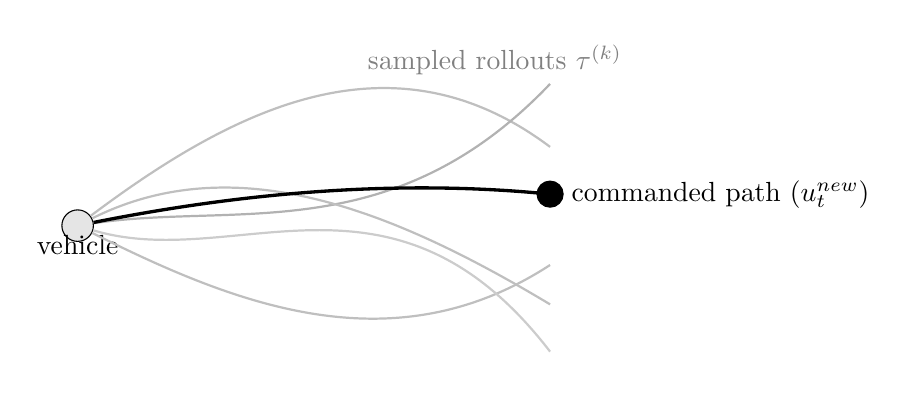
\begin{tikzpicture}[scale=1.0]
    \node[draw,circle,fill=gray!20,minimum size=0.4cm] (start) at (0,0) {};
    \node[below] at (start) {vehicle};

    \draw[gray!50, thick] (start) .. controls (2,1.5) and (4,2.5) .. (6,1.0);
    \draw[gray!50, thick] (start) .. controls (2,-1.0) and (4,-1.8) .. (6,-0.5);
    \draw[gray!60, thick] (start) .. controls (2,0.3) and (4,-0.3) .. (6,1.8);
    \draw[gray!40, thick] (start) .. controls (2,-0.6) and (4,1.0) .. (6,-1.6);
    \draw[gray!50, thick] (start) .. controls (2,1.0) and (4,0.2) .. (6,-1.0);

    \draw[very thick] (start) .. controls (2,0.4) and (4,0.6) .. (6,0.4);
    \node[draw,circle,fill=black,minimum size=0.15cm] at (6,0.4) {};
    \node[right] at (6.15,0.4) {commanded path ($u_t^{\text{new}}$)};

    \node[gray] at (5.3,2.1) {sampled rollouts $\tau^{(k)}$};
  \end{tikzpicture}
  \caption[MPPI's sampling-based control update]{MPPI's sampling-based control update: $K$ randomly perturbed control sequences are each rolled forward through the vehicle model into a candidate trajectory $\tau^{(k)}$ (grey), each scored by the total critic cost $S(\tau^{(k)})$; Equation~\ref{eq:mppi-weight}'s softmax weighting then combines all $K$ trajectories into one commanded control sequence (black). Lower-cost rollouts contribute more weight, but every sampled trajectory contributes something, unlike a hard arg-min over a discrete set of candidates.}
  \label{fig:mppi-concept}
\end{figure}

\subsection{AMCL's Particle Filter and Recovery Mechanism in Detail}
\label{sec:amcl-math}

AMCL maintains its belief about the robot's pose as a set of $N$
weighted particles $\{(x^{(i)}, w^{(i)})\}_{i=1}^{N}$, each a
concrete pose hypothesis, updated on every new odometry/LiDAR pair
through the standard Monte Carlo localisation prediction-update-resample
cycle \cite{thrun2000probrob}:

\begin{enumerate}
  \item \textbf{Prediction (motion model).} Each particle is
    propagated forward using the commanded/odometric motion since the
    last update, corrupted by noise whose magnitude is controlled by
    the $\alpha_1$--$\alpha_4$ parameters mentioned in the component
    list above (roughly: $\alpha_1$/$\alpha_2$ scale rotational noise
    from the odometry's rotational and translational components
    respectively, $\alpha_3$/$\alpha_4$ scale translational noise the
    same way). Larger values inject more particle spread per unit of
    commanded motion, modelling greater distrust in odometry.
  \item \textbf{Update (measurement model).} Each particle's weight
    is set proportional to the likelihood of the actual LiDAR scan
    given that particle's hypothesised pose and the static map,
    typically via a likelihood-field model that scores each scan
    endpoint by its proximity to the nearest mapped obstacle from that
    hypothesised pose.
  \item \textbf{Resampling.} A new particle set is drawn, with
    replacement, with probability proportional to weight. Particles
    consistent with the actual scan multiply, while inconsistent ones
    are discarded. The particle cloud then statistically converges
    toward the true pose over repeated cycles. AMCL's ``adaptive'' element
    (KLD-sampling) additionally varies $N$ itself between update
    cycles, using fewer particles once the distribution is already
    tightly converged and more while it remains spread out.
\end{enumerate}

\begin{figure}[htbp]
  \centering
  \begin{tikzpicture}[
      block/.style={draw, rectangle, rounded corners, minimum height=1.1cm, minimum width=3.4cm, align=center, font=\small},
      arr/.style={-{Latex[length=2mm]}, thick}
    ]
    \node[block] (predict) at (0,0) {1. Prediction\\(motion model)};
    \node[block] (update) at (5,0) {2. Update\\(measurement model)};
    \node[block] (resample) at (2.5,-1.8) {3. Resampling};

    \draw[arr] (predict) -- (update);
    \draw[arr] (update) -- (resample);
    \draw[arr] (resample.west) .. controls (-1.2,-1.1) and (-1.2,-0.5) .. (predict.south west);

    \draw[arr] (-0.2,1.3) -- (predict.north) node[midway,left,align=right] {odometry};
    \draw[arr] (5.2,1.3) -- (update.north) node[midway,right,align=left] {LiDAR scan\\+ map};
  \end{tikzpicture}
  \caption{The AMCL particle filter's prediction-update-resampling cycle, repeated on every new odometry/LiDAR pair (Section~\ref{sec:amcl-math}).}
  \label{fig:amcl-cycle}
\end{figure}

The parameters directly responsible for the freeze failure mode
documented in Section~\ref{sec:ruled-out} are a separate pair from
the four motion-model $\alpha$s above.
\texttt{recovery\_alpha\_slow}/\texttt{recovery\_alpha\_fast} govern
an \emph{augmented} MCL recovery mechanism: injecting randomly
sampled particles when recent localisation quality drops. This
general concept was evaluated directly against the alternative of
plain MCL, for exactly this kidnapped-robot/recovery scenario, in
\cite{thrun2001robustmcl}.

AMCL's specific implementation of the concept, read directly from
its own parameter documentation and used as configured throughout
this thesis, tracks two exponential moving averages of the particle
set's average weight: a slow long-run average $\bar{w}_{\text{slow}}$
and a fast short-run average $\bar{w}_{\text{fast}}$. Both are
updated after every measurement step, as

\begin{equation}
  \bar{w}_{\text{slow}} \mathrel{+}= \alpha_{\text{slow}}\left(\bar{w} - \bar{w}_{\text{slow}}\right), \qquad
  \bar{w}_{\text{fast}} \mathrel{+}= \alpha_{\text{fast}}\left(\bar{w} - \bar{w}_{\text{fast}}\right),
  \label{eq:amcl-recovery}
\end{equation}

where $\bar{w}$ is the current cycle's average particle weight.

During resampling, instead of drawing every new particle from the
existing weighted set, each new particle is drawn \emph{uniformly at
random from the entire map} with probability $\max\!\left(0,\ 1 -
\bar{w}_{\text{fast}}/\bar{w}_{\text{slow}}\right)$. Intuitively: if
recent particle quality ($\bar{w}_{\text{fast}}$) has dropped
noticeably below the longer-run baseline ($\bar{w}_{\text{slow}}$),
the filter injects fresh, unbiased hypotheses to help it recover
from a bad convergence or a ``kidnapped robot'' scenario, rather than
continuing to resample only from a particle set that may have
already converged to the wrong pose.

This project's simulation-tuned configuration originally inherited
$\alpha_{\text{slow}} = \alpha_{\text{fast}} = 0.0$. At that setting,
neither running average is ever updated from its initial value, so
the random-injection probability is permanently fixed rather than
responsive to real degradation in particle quality. A clean
simulation rarely needs this recovery path at all, but on real,
non-ideal sensor noise, the particle set can converge overconfidently
to an incorrect pose with no mechanism available to reintroduce
diversity. This is the permanent freeze Section~\ref{sec:ruled-out}
reports and fixes, by raising these two parameters off zero.

\section{The Quanser QCar Platform}
\label{sec:qcar-platform}

The physical platform underlying this thesis is the Quanser QCar:
the original platform, not the newer, distinct QCar~2 that Quanser's
documentation set also covers. It is a 1/10th-scale rear-wheel-drive,
Ackermann-steered research vehicle \cite{quanser2023qcar}.

Its onboard computer is an NVIDIA Jetson TX2 system-on-module,
running Ubuntu 18.04 LTS with 32\,GB eMMC storage and Python~3.6.9.
It ships with both ROS~1 Melodic and ROS~2 Dashing pre-installed
side by side, though neither is auto-sourced in the default shell
environment.

The platform additionally ships with an Intel RealSense D435 RGBD
camera, four 360\textdegree{} CSI cameras and an onboard IMU as
standard hardware. This thesis's navigation pipeline uses none of
these. It relies solely on the 2D LiDAR for mapping, localisation
and obstacle sensing, with pose estimation between LiDAR updates
coming from wheel-encoder-based odometry rather than the IMU.

The IMU is electrically present and exposed by QCar's HAL/PAL
library (\texttt{gyroscope/}\allowbreak\texttt{accelerometer} fields), but
nothing in this project's software stack reads it. Cartographer's
\texttt{use\_imu\_data} is left \texttt{false}. No IMU sensor
plugin is declared in the simulation's URDF either, so only the
LiDAR is discussed further.

\begin{figure}[htbp]
  \centering
  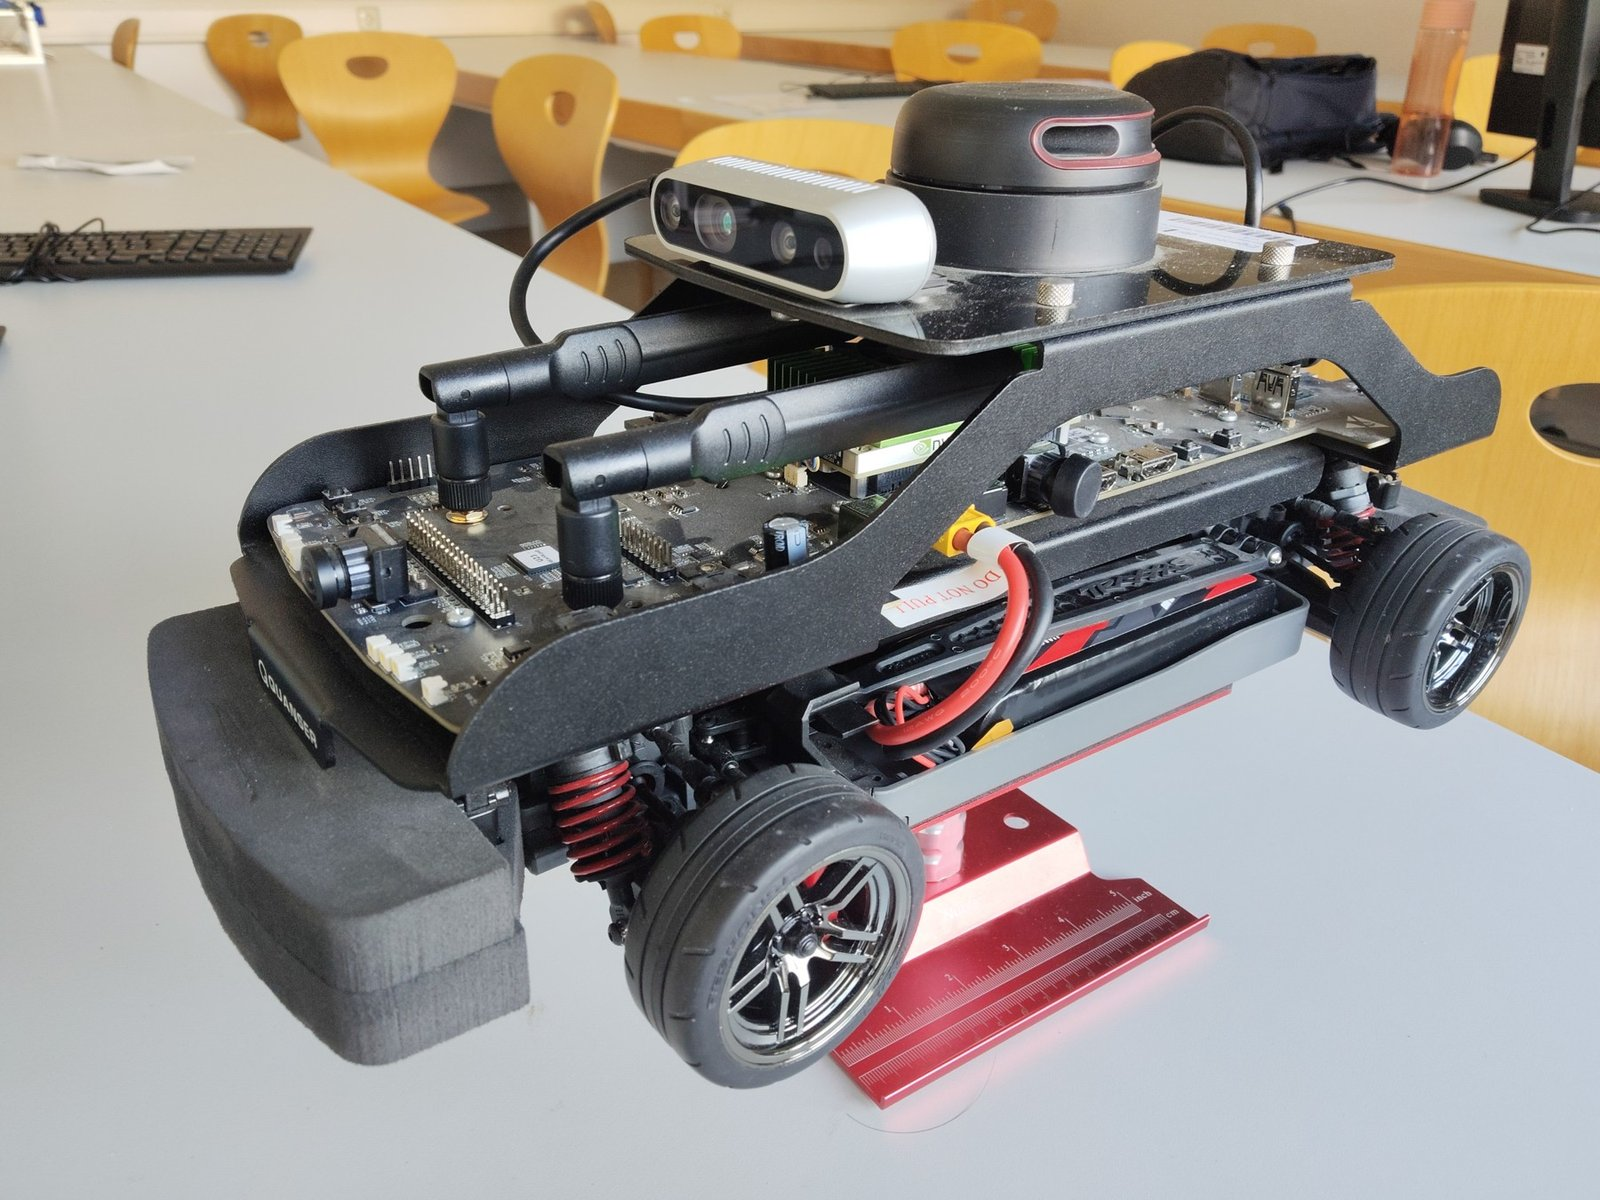
\includegraphics[width=0.75\textwidth]{figures/qcar-sensors-battery-photo.jpg}
  \caption{The Quanser QCar platform used throughout this thesis, raised off the ground.}
  \label{fig:qcar-sensors-battery-photo}
\end{figure}

Drive and steering actuation are exposed through Quanser's own
Hardware Abstraction Layer / Product Application Layer (HAL/PAL)
Python library, which wraps the vehicle's motor, servo, encoder and
battery-monitoring hardware behind a \texttt{QCar} object exposing
\texttt{read()}/\texttt{write()} calls. Two of its limits are enforced
at the field-programmable gate array (FPGA) level regardless of what
software commands \cite{quanser2023qcar}. The steering command range
is $\pm 0.5$~rad against a physical limit of $\pm 0.5236$~rad
($\pm\ang{30}$). An overcurrent protection state, triggered at
5\,A/8\,s, 10\,A/2\,s or 15\,A/0.5\,s, forces the vehicle into a
neutral mode until the underlying hardware-in-the-loop device is
restarted. Both limits are respected throughout every piece of
drive-control code presented in this thesis.

A third figure, commonly listed alongside these two, is not a
hardware-enforced limit at all. Quanser's own troubleshooting
documentation \emph{recommends} saturating commanded PWM duty cycle
to $\pm 30\%$ with a $100\%/\mathrm{s}$ rate limiter, specifically to
avoid a battery-brownout-induced shutdown
\cite{quanser2023troubleshooting} -- not something the HAL itself
clamps. This project's own drive-control code adopts that
recommendation (Section~\ref{sec:final-calibration}'s
\texttt{THROTTLE\_LIMIT}), but it is a software policy choice, not a
property of the vehicle the way the other two limits are.

A property of the HAL library specific to this platform and central
to one of this thesis's most significant findings
(Section~\ref{sec:readmode-bug}) is its two supported I/O modes. In
\emph{immediate I/O} (\texttt{readMode=0}), each call to
\texttt{read()} triggers a fresh hardware sample. In \emph{task-based
I/O} (\texttt{readMode=1}), a background acquisition task begins
sampling into a fixed-depth ring buffer at object construction time,
independently of when (or whether) the caller ever calls
\texttt{read()}. This distinction is not merely an implementation
detail. Chapter~\ref{ch:calibration} documents how it produced a
measurement artefact large enough and stable enough to be
repeatedly and reasonably misattributed to genuine vehicle physics
before its true cause was found.

\section{The Sim-to-Real Gap}
\label{sec:sim-to-real-concept}

The term \emph{sim-to-real gap} (or \emph{reality gap}) is most
extensively studied in the deep-reinforcement-learning literature,
where it refers to the degradation of a policy's performance when a
controller trained purely in simulation is transferred to a physical
robot \cite{zhao2020sim2real}. This thesis borrows the term for a
broader, classically-engineered sense not specific to any learned
policy: any systematic discrepancy between a robot's simulated and
physical behaviour under nominally identical software and commands.
Sources of this gap are commonly grouped into a few broad categories,
all of which recur, in concrete and specific form, across this
thesis's methodology chapters:

\begin{itemize}
  \item \textbf{Unmodelled or under-modelled physical effects} --
    e.g.\ static friction / stiction, actuator response lag or
    non-linear actuator-to-output mappings that a simulator either
    omits entirely or models only in idealised form. Chapter~\ref{ch:calibration}'s
    throttle calibration and friction-deadband findings are a direct
    instance of this category.
  \item \textbf{Sensor and estimation differences} -- simulated
    sensors are frequently noiseless or near-noiseless and
    perfectly time-synchronised with the simulation clock, whereas
    physical sensors carry real noise, real latency and, in a
    distributed system, real inter-process clock skew.
    Chapter~\ref{ch:hardware-bridge}'s clock-offset and LiDAR
    angle-convention fixes fall into this category.
  \item \textbf{Software/communication-layer differences} -- a
    simulated robot typically runs its entire software stack as
    co-located ROS~2 processes on one machine. A physical robot may
    be split across incompatible middleware versions, unreliable
    wireless links or, as found directly in this project, firmware-
   or driver-level buffering that a simulation has no equivalent of
    at all. Chapters~\ref{ch:hardware-bridge}
    and~\ref{ch:calibration} both document findings in this
    category.
\end{itemize}

A methodological point recurs throughout this thesis and is made
explicit here because it shapes every later chapter's approach:
these categories are not always distinguishable from the symptom
alone. A fixed-duration, speed-independent delay between a software
command and its physical effect is, from a black-box measurement
standpoint, equally consistent with several explanations. It could
be drivetrain coasting, a physical-effect explanation or a
command-delivery lag in the bridge software, a communication-layer
explanation. Or, as this thesis's own investigation ultimately
found, it could be a stale-data artefact in a sensor read path -- a
sensor/estimation-layer explanation that happens to mimic a physical
one almost exactly.

Distinguishing between these required, in every case documented in
this thesis, going beyond the symptom to a direct measurement or
source-level inspection of the specific layer under suspicion. This
is a theme Chapter~\ref{ch:calibration} returns to explicitly.
